\documentclass{article}
\usepackage{v-test-paper}
%\geometry{paperwidth=6 in, paperheight=3.375 in, left=7 mm, right=7 mm, top=2 mm, bottom=18 mm}

\newenvironment{solution}{\color{red!85!black}}{}
%\excludecomment{solution}
\title{Distance}
\begin{document}
\maketitle

\begin{center}
    \begin{quote}
        \textit{Actual path length of a trajectory traversed by a particle is called distance.}
    \end{quote}
\end{center}

\begin{center}
    \begin{tikzpicture}
        \def\tat{3.6}%tangent at {x}
        \def\dx{0.2}%tangent at {x}
            \tzaxes(-0.5, -0.5)(7,4){$x$}{$y$}
            \tztos"curve"
                (0,0)[out=0, in=-180]
                (3,1.5)[out=0, in=-180]
                (6, 3.5);
                
            \tzvXpointat{curve}{\tat-\dx}(A)
            \tzvXpointat{curve}{\tat+\dx}(B)
            \tztangentat[->]"TL"{curve}{\tat}[\tat-0.15:4.5]{$\vec{v}$}
            % \tzcoor*($($(A)!0.5!(B)$)!1cm!90:(B)$)(O){$O$}[ar]
            %\tzXpoint{normal}{normall}(X)
            % \tzcircle[dashed](O)(1)
            % \tzline[dashed, red](O)(A)
            % \tzline[dashed, red](O)(B)
            \tzcoor($(A)+(2*\dx, 0)$)(C)
            \tzline(A)(C){$\d{x}$}[mb, scale=0.75]
            \tzline(B)(C){$\d{y}$}[mr, scale=0.75]
    \end{tikzpicture}
\end{center}
    \begin{align*}
        \intertext{We took a small segment($\d{l}$) along the curve, assuming this segment as hypotenuse we can construct a small right angle triangle with base $\d{x}$ and height $\d{y}$}
        \d{l}^2 &= \d{x}^2 + \d{y}^2\\
        \intertext{$\d{x}$ can be expressed as $v_x \d{t}$ and $\d{y}$ can be expressed as $v_y \d{t}$}
        \d{l}^2 &= (v_x \d{t})^2 + (v_y \d{t})^2\\
        \d{l} &= \sqrt{\left(v_x^2 + v_y^2 \right)\d{t}^2}\\
        \intertext{The total distance traversed by the particle is the sum of all the small segments}
        \int \d{l} &= \int |\vec{v}|\d{t}\\  
        \textit{Distance } &= \int |\vec{v}|\d{t}\\
    \end{align*}

    \begin{center}
        \textsc{Velocity-time graph}
    \end{center}
    \begin{center}
        \begin{tikzpicture}
            \tzaxes(-0.5, -2)(7,2){$t$}{$v$}
            \def\Fx{0.2*(\x-1)^2-1}
            \tzfn\Fx[0:5.25]
            \tzfnarea*[pattern=north west lines, opacity=0.8]{\Fx}[0:5]
            \tzhXpoint{Fx}(1,0)(T1)
            
            \tznode(T1){$t_1$}[b]
            \tznode(5, 0){$t_2$}[b]
        \end{tikzpicture}
    \end{center}
    \begin{align*}
        \intertext{The magnitude of area under the velocity-time graph gives the distance traversed by the particle.}
        \textit{distance } &= \int_{0}^{t_2} |\vec{v}|\d{t} = \left|\int_{0}^{t_1} \vec{v}\d{t}\right| + \left|\int_{t_1}^{t_2} \vec{v}\d{t}\right|\\
    \end{align*}

    Distance travelled by a particle in a straight line
    \begin{center}
        \begin{tikzpicture}
            \tzcoor*(0, 0)(O){$O$}[b]
            \tzcoor*(6, 0)(A){$A$}[b]
            \tzline[-->--](O)(A)
            \tzline+[->]<0, -0.5>($(O)!0.35!(A)$)(1, 0){$v(+)$}[r]
            \tzline+[->]<0, -0.5>($(O)!0.65!(A)$)(5, 0){$v(-)$}[r]
        \end{tikzpicture}
    \end{center}

    \begin{center}
        \textsc{Modulus}
    \end{center}
    \begin{align*}
        \intertext{The modulus of a number is the positive value of the number}
        |x| &= \begin{cases}
            x & \text{if } x \geq 0\\
            -x & \text{if } x < 0
        \end{cases}
    \end{align*}



\pagebreak 


\begin{center}
    \textsc{Illustrations}
\end{center}
\begin{enumerate}
    \item The velocity of a particle moving in a straight line is given by $v=t-2$ where $v$ is in m/s and $t$ is in seconds. Find the distance travelled by the particle in the first 4 seconds.\\
    \begin{solution}
        $\Rightarrow$
        \begin{align*}
            \intertext{The distance travelled by the particle is given by}
            \textit{Distance } &= \int_{0}^{4} |t-2|\d{t}\\
            |t-2| &= \begin{cases}
                t-2 & \text{if } t \geq 2\\
                -(t-2) & \text{if } t < 2
            \end{cases}\\
            &= \int_{0}^{2} (2-t)\d{t} + \int_{2}^{4} (t-2)\d{t}\\
            &= \left[2t-\frac{t^2}{2}\right]_{0}^{2} + \left[\frac{t^2}{2}-2t\right]_{2}^{4}\\
            &= \left[4-2\right] + \left[(8-8)-(2-4)\right]\\
            &= 4\m
        \end{align*}
        Alternatively, the distance travelled by the particle can be calculated by finding the area under the velocity-time graph.
        \begin{center}
            \begin{tikzpicture}
                \tzaxes(-0.5, -2.5)(6,2.5){$t$}{$v$}
                \def\Fx{\x-2}
                \tzfn\Fx[0:4.5]
                \tzfnarea*[pattern=north west lines, opacity=0.8]{\Fx}[0:4]
                \tzhXpoint{Fx}(2,0)(T1)
                \tzticks{2/$2$, 4/$4$}{-2/$-2$, 2/$2$}
            \end{tikzpicture}
        \end{center}
        \begin{align*}
            \textit{Distance } &= \dfrac{1}{2}\cdot 2 \cdot 2 + \dfrac{1}{2}\cdot 2 \cdot 2\\
            &= 4\m
        \end{align*}
        \begin{center}
            \begin{tikzpicture}
                \tzcoor*(0, 0)(O){$t=0, v<0$}[b]
                \tzcoor*(-4, 0)(A){$t=2, v=0$}[b]
                \tzline[-->--](O)(A)
                \tzline[-->--]<0, 0.5>(A)(0, 0){$t>2, v>0$}[ma]
            \end{tikzpicture}
        \end{center}
    \end{solution}

    \item A particle moves along the x-axis according to the equation $x=A\cos(\omega t)$. Find the distance travelled by the particle during the time interval $t=0$ to $t=t$.\\
    \begin{solution}
        $\Rightarrow$
        \begin{align*}
            \intertext{The velocity of the particle is given by}
            v &= \dfrac{\d{x}}{\d{t}}\\
            &= -A\omega\sin(\omega t)\\
            \intertext{The distance travelled by the particle is given by}
            \textit{Distance } &= \int_{0}^{t} |v|\d{t}\\
            &= \int_{0}^{t} |-A\omega\sin(\omega t)|\d{t}\\
            |-A\omega\sin(\omega t)| &= \begin{cases}
                -A\omega\sin(\omega t) & \textit{if \quad} -A\omega\sin(\omega t) \geq 0\\
                A\omega\sin(\omega t) & \textit{if \quad} -A\omega\sin(\omega t) < 0
            \end{cases} \\  
            &= \begin{cases}
                -A\omega\sin(\omega t) & \textit{if \quad} \sin(\omega t) \leq 0\\
                A\omega\sin(\omega t) & \textit{if \quad} \sin(\omega t) > 0
            \end{cases}\\
            &= \begin{cases}
                -A\omega\sin(\omega t) & \textit{if \quad} (2n-1)\pi \lMeq \omega t \leq (2n\pi)\\
                A\omega\sin(\omega t) & \textit{if \quad} \sin(\omega t) > 0
            \end{cases}\\ 
        \end{align*}
    \end{solution}

\end{enumerate}







\end{document}